\documentclass{beamer}
\usepackage{listings}
\usetheme{Copenhagen}
\usecolortheme{beaver}
\setbeamertemplate{navigation symbols}{}
\setbeamertemplate{footline}{\parbox[t][12pt][c]{12pt}{~\scriptsize\insertframenumber}}
% \usepackage{beamerthemesplit} // Activate for custom appearance

%%%%%%%%%%%%
% MVS: Language definitions
%
\renewcommand{\ttdefault}{pcr}
\lstset{
  basicstyle=\small\ttfamily,
  breaklines=true
}
\lstdefinelanguage{cvl}{
  morekeywords={generalize,to, with, other, at, zoom, levels, weigh, by, subject, and, create, constraint, as, not, exists, resolve, if, delete, select, from, where, in, order, over, setup, teardown,force,min,level,for,allornothing,join,on,setup,group,having,index,temporary,table,drop,partition,merge,partitions},
  sensitive=false,
  morecomment=[l]{//},
  morecomment=[s]{/*}{*/},
  morestring=[b]",
}
\lstset{
  language=cvl
}


\title{Declarative Cartography}
\subtitle{In-Database Map Generalization of Spatial Datasets}
\author{\underline{Pimin Konstantin Kefaloukos}, Marcos Vaz Salles, \\Martin Zachariasen\\ \small{\emph{Computer Science Department (DIKU)}, \textbf{University of Copenhagen}}}

\date{\today}

\begin{document}

\frame{\titlepage}

\frame
{
  \frametitle{Motivation}
  \begin{itemize}
  \item \textbf{Imagine}: you're a \emph{data journalist} and want to tell a story about restaurants in Z\"{u}rich \emph{using a map}.
  \item \textbf{Database}: You have a \emph{database} of restaurants (unique ID, location, star rating, name etc.)
  \item Simply showing all the records creates a mess (see picture)
  \item Generalization of thematic data is an important problem, with increasing use cases in \emph{social networks}, \emph{data journalism} etc
  \end{itemize}
  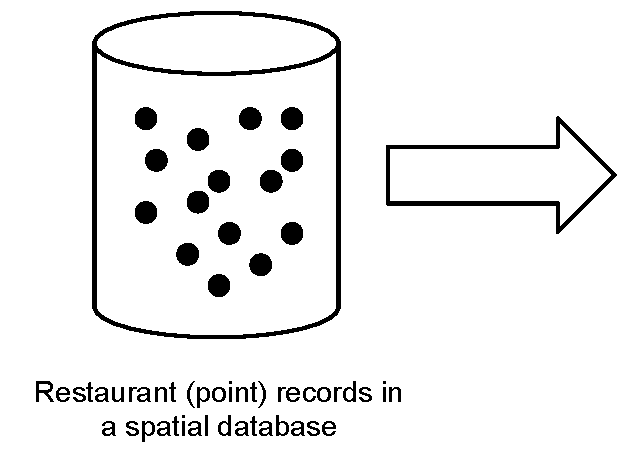
\includegraphics[scale=0.5]{figs/spatial-database-with-points.pdf} 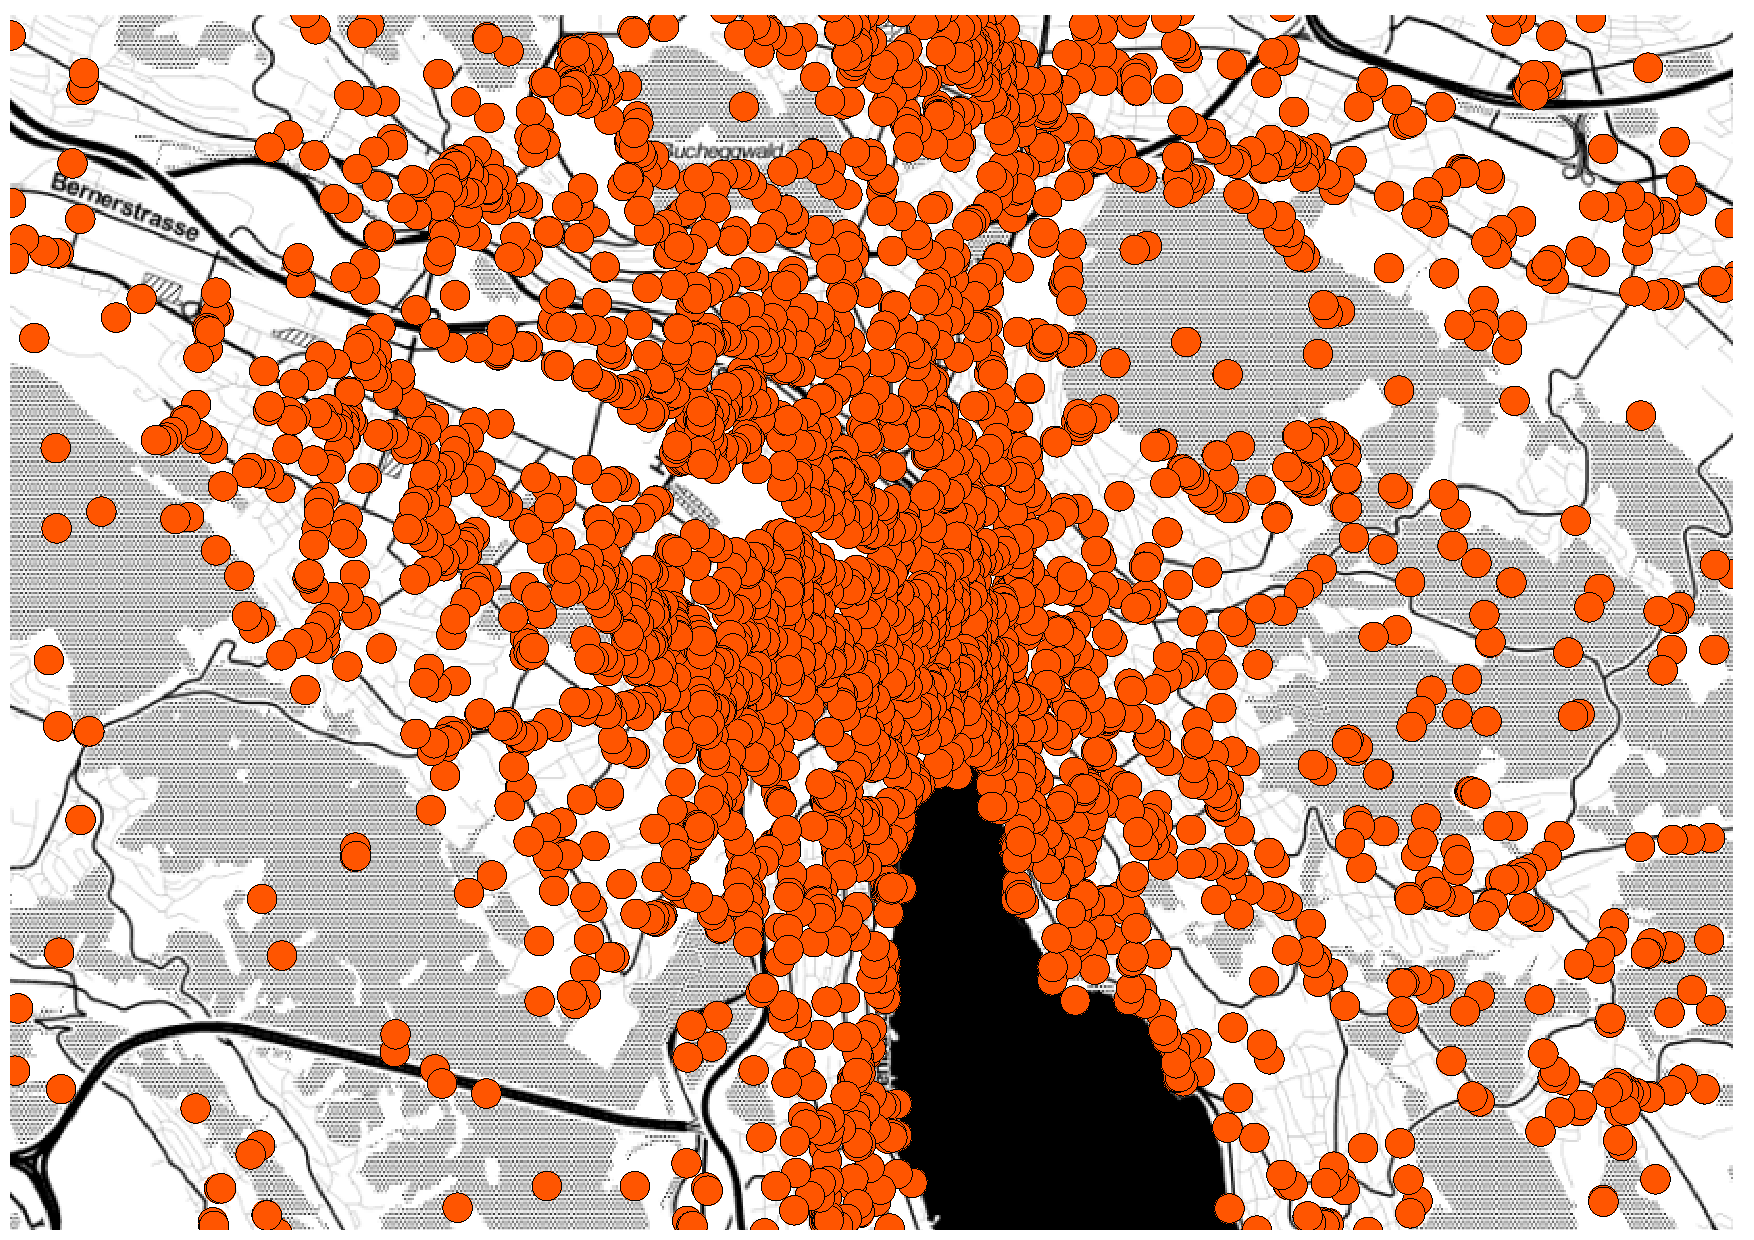
\includegraphics[scale=0.18]{figs/zurich-unfiltered.pdf}
}

% Setting stage
\frame[t]
{
  \frametitle{What a good (thematic) map might look like}
\begin{columns}[t]
	\begin{column}[l]{6cm}
		\begin{itemize}[<+->]
			\item Records should appear \emph{gradually} when zooming in, i.e. \emph{constant information~density}
			\item ``Important'' records should get priority
			\item Visible records should \emph{remain visible} when zooming in
			\item There should be some way of imposing \emph{constraints}, e.g. ``records not too close''
		\end{itemize}
	\end{column}
	\begin{column}[l]{6cm}
    \begin{figure}
    	\vspace{-1.5em}
	After generalization: \\
    	\includegraphics<1>[scale=0.17]{figs/zoom12.pdf}
        \includegraphics<2>[scale=0.17]{figs/zoom13.pdf}
        \includegraphics<3>[scale=0.17]{figs/zoom14.pdf}
        \includegraphics<4>[scale=0.17]{figs/zoom15.pdf}\\
        Before generalization:\\
        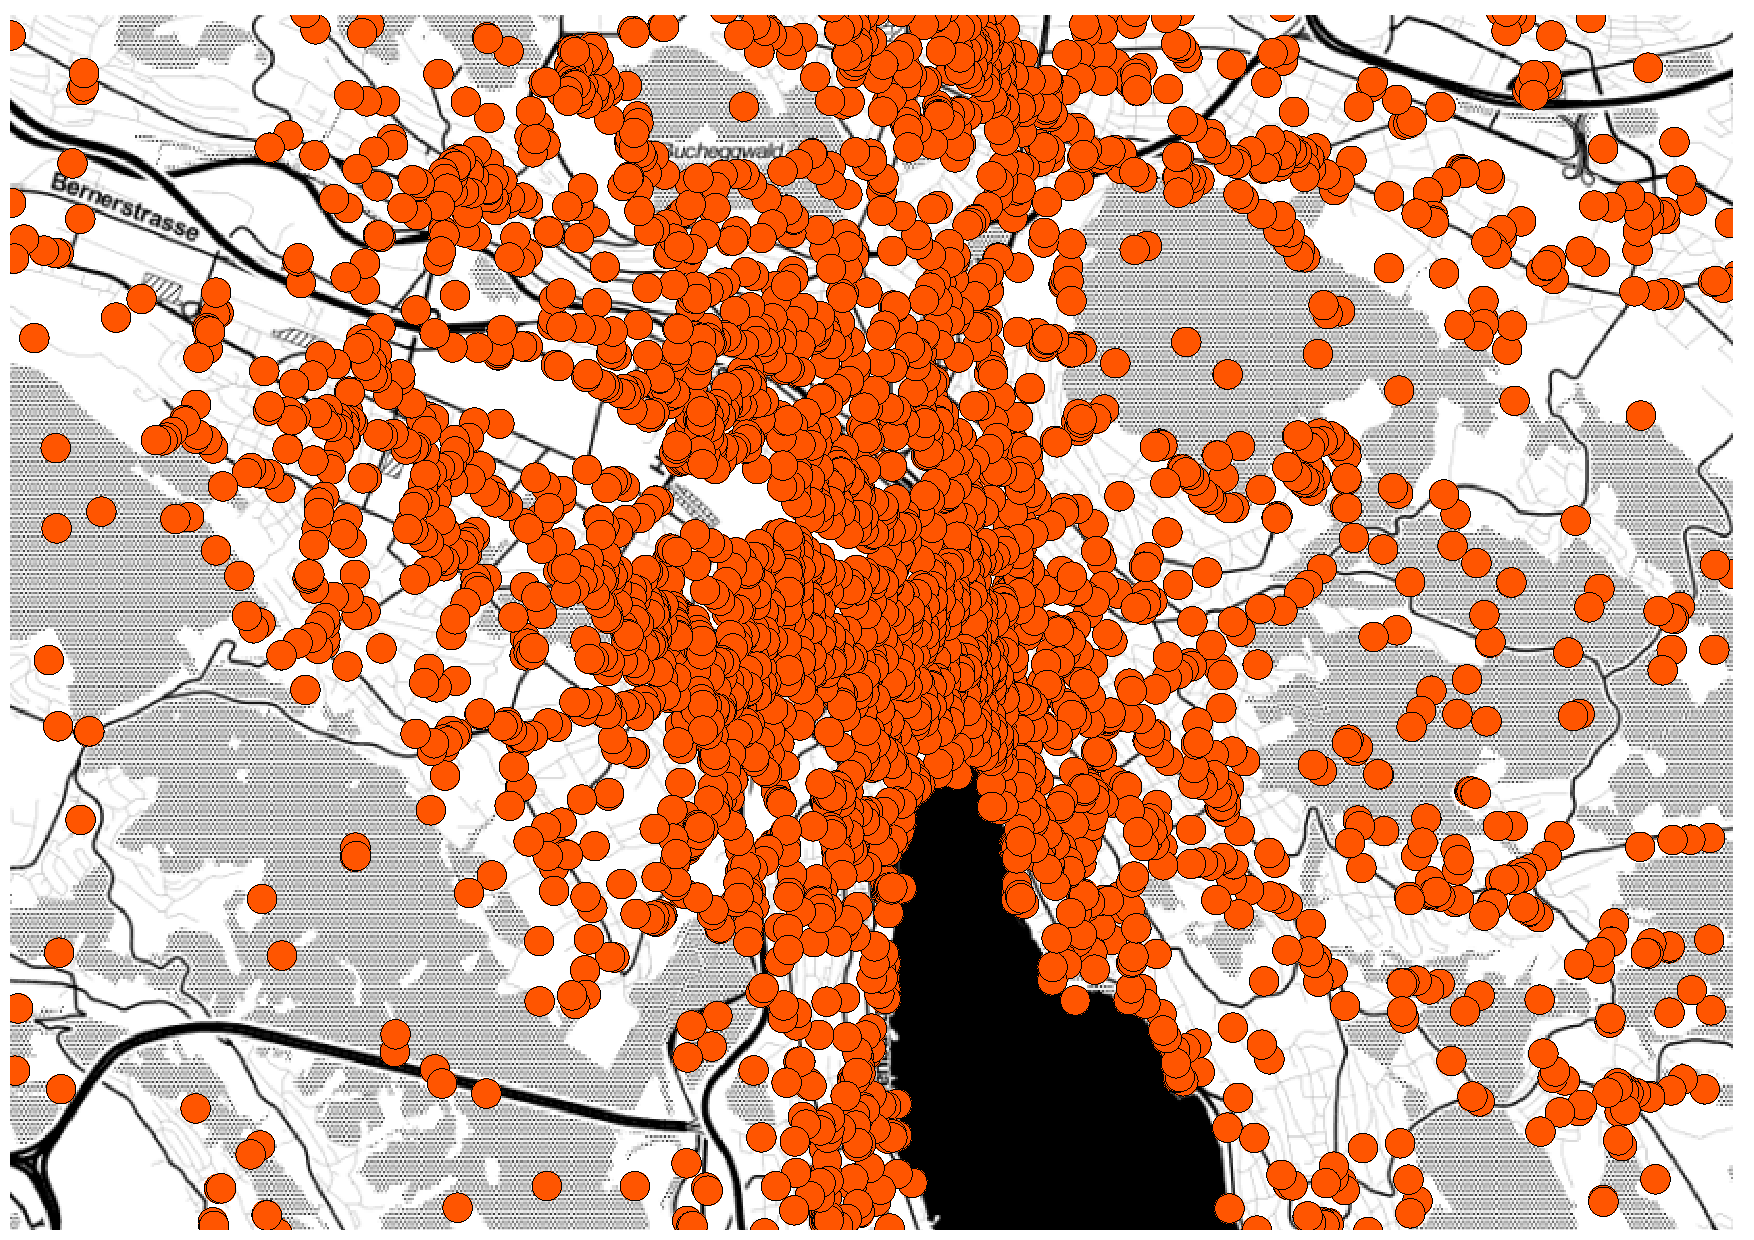
\includegraphics[scale=0.13]{figs/zurich-unfiltered.pdf}\\
    \end{figure}                            
\end{column}
\end{columns}
}

% What we will achieve
\frame[t]
{
  \frametitle{What we mean by generalization}
	\begin{itemize}[<+->]
		\item \textbf{Input}: table with \texttt{ID}, \texttt{Geometry} and additional columns
		\item \textbf{Output} : input table extended with \texttt{MinZoom} column
		\item Value of \texttt{MinZoom} is the zoom level $z \in \lbrack 1, \mathcal{Z} \rbrack$ when a record should become visible in the map
		\item Assignment of values to \texttt{MinZoom} corresponds to a particular generalization of the data
		\item $O(\mathcal{Z}^n)$ many ways to assign a value to \texttt{MinZoom} for $n$ records
	\end{itemize}
	\vspace{1em}
	\begin{columns}[t]
		\begin{column}[l]{4cm}
  		\includegraphics<1>[scale=0.35]{figs/cvl-table-before-after.pdf}
		\includegraphics<2>[scale=0.35]{figs/cvl-table-before-after-2.pdf}
		\includegraphics<3>[scale=0.35]{figs/cvl-table-before-after-2.pdf}
		\includegraphics<4>[scale=0.35]{figs/cvl-table-before-after-2.pdf}
		\includegraphics<5>[scale=0.35]{figs/cvl-table-before-after-2.pdf}
		\end{column}
		\begin{column}[r]{4cm}
		\includegraphics<3>[scale=0.30]{figs/cvl-problem.pdf}
		\includegraphics<4>[scale=0.30]{figs/cvl-problem.pdf}
		\includegraphics<5>[scale=0.30]{figs/cvl-problem.pdf}
		\end{column} 
  	\end{columns}
}

% Setting stage
\frame[t]
{
  \frametitle{Spatial databases}
	\begin{itemize}[<+->]
		\item Spatial data is often stored in a \emph{spatial database}
		\item Databases have powerful capabilities
		\item \emph{joins}, \emph{sorting}, \emph{spatial indexing} and \emph{spatial functions}
	\end{itemize}
	\begin{center}
	\begin{figure}
    		\includegraphics<1>[scale=0.3]{figs/cvl-powerful-database.pdf}
    		\includegraphics<2>[scale=0.3]{figs/cvl-powerful-database.pdf}
		\includegraphics<3>[scale=0.3]{figs/cvl-powerful-database-2.pdf}
	\end{figure}       
	\end{center}                     
}

\frame[t]
{
  \frametitle{Situation}
	\begin{itemize}[<+->]
		\item Generalization algorithms are usually implemented in \emph{external software}
		\item After processing the data we put back into the database
		\item Treats the database as ``dumb'' storage until query time
		\item But remember, databases are really quite powerful
	\end{itemize}
	\begin{center}
	\begin{figure}
    		\includegraphics<1>[scale=0.3]{figs/cvl-external-software-out.pdf}
		\includegraphics<2>[scale=0.3]{figs/cvl-external-software-in.pdf}
		\includegraphics<3>[scale=0.3]{figs/cvl-external-software-rest.pdf}
		\includegraphics<4>[scale=0.3]{figs/cvl-powerful-database-2.pdf}
	\end{figure}       
	\end{center}                     
}

\frame{
	\frametitle{Recycle technology: databases}
	\begin{center}
	
\includegraphics[scale=0.88]{figs/wall-e.jpg}
	\end{center}
}


\frame[t]
{
  \frametitle{Why not use the database to generalize data?}
	\begin{itemize}[<+->]
		\item We could formulate \emph{goal} of generalization in a ``high-level'' language
		\item Translate high-level program to low-level database program that generalizes data
		\item Moving \textbf{code-to-data} instead of data-to-code
		\item This is what we did :-)

	\end{itemize}
	\begin{center}
	\begin{figure}
    		\includegraphics<1>[scale=0.3]{figs/cvl-state-intension.pdf}
    		\includegraphics<2>[scale=0.3]{figs/cvl-compile-statement.pdf}
		\includegraphics<3,4>[scale=0.3]{figs/cvl-code-to-data.pdf}
	\end{figure}       
	\end{center}                     
}

% Introduce syntax
\begin{frame}[fragile,t]
  \frametitle{High-level language: \texttt{GENERALIZE} statement}
  \begin{center}
  \fbox{What users write}
  \end{center}
  \begin{description}[<+->]
  \item[Input and output]:
  \begin{lstlisting}
GENERALIZE restaurants 
TO restaurants2
\end{lstlisting}
  \item[How many zoom levels?]:
\begin{lstlisting}
AT 20 ZOOM LEVELS
\end{lstlisting}
  \item[How should records be prioritized?]:
\begin{lstlisting}
WEIGH BY star_rating
\end{lstlisting}
  \item[What spatial constraints should be enforced?]:
\begin{lstlisting}    
SUBJECT TO proximity 10 AND density 64
\end{lstlisting}
\end{description}
\end{frame}

\begin{frame}[fragile]
\frametitle{High-level language: \texttt{CREATE CONSTRAINT}}

  \begin{center}
  \fbox{What expert users write}
  \end{center}

\begin{description}[<+->]
\item[Give the constraint a name]:
\begin{lstlisting}[escapechar=@]
CREATE CONSTRAINT {@name as string@}
\end{lstlisting}
\item[How is the constraint condition defined?]:
\begin{lstlisting}[escapechar=@]
AS NOT EXISTS (
  {@SQL@}
)
\end{lstlisting}
\item[How to resolve with constraint violations?]:
\begin{lstlisting}[escapechar=@]
RESOLVE cid IF DELETE (
  {@SQL@}
)
\end{lstlisting}
\end{description}
\end{frame}

% Introduce syntax
%\begin{frame}[fragile]
%  \frametitle{Embedded SQL}
%  \begin{center}
%  \fbox{Generalize statement}
%  \end{center}
%  We reuse SQL as an embedded language to gain expressibility
%  \vspace{1.5em}
%  \begin{lstlisting}[escapechar=@]
%GENERALIZE {@SQL FROM clause@} 
%...
%...
%WEIGH BY {@float-valued SQL expression@}
%...
%\end{lstlisting}
%\end{frame}


%\begin{frame}[fragile]
%\frametitle{High-level language: \texttt{CREATE CONSTRAINT}}
%
%  \begin{center}
%  \fbox{Create constraint statement}
%  \end{center}
%
%\begin{description}[<+->]
%\item[Give the constraint a name]:
%\begin{lstlisting}[escapechar=@]
%CREATE CONSTRAINT {@name as string@}
%\end{lstlisting}
%\item[How is the constraint condition defined?]:
%\begin{lstlisting}[escapechar=@]
%AS NOT EXISTS
%  {@SQL SELECT statement@}
%\end{lstlisting}
%\item[How to resolve with constraint violations?]:
%\begin{lstlisting}[escapechar=@]
%RESOLVE cid IF DELETE (
%  {@SQL integer expression@}
%)
%\end{lstlisting}
%\end{description}
%\end{frame}

\frame{
	\frametitle{Constraints explained}
	
	\textbf{Example}: Proximity constraint
	\vspace{0.5em}
	\begin{itemize}[<+->]
	\item Constraints defined by defining what a ``conflict'' means
	\item Set of records that don't \emph{fit} on the same zoom-level
	\item Proximity constraint: resolve a conflict by ``deleting'' one or the other record
	\vspace{0.5em}
	\end{itemize}
	\begin{center}
  		\includegraphics<1,2>[scale=0.35]{figs/cvl-proximity-conflicts-1.pdf}
		\includegraphics<3>[scale=0.35]{figs/cvl-proximity-conflicts-2.pdf}
  	\end{center}

}

%\frame{
%	\frametitle{Division of labour}
%	\begin{itemize}[<+->]
%	\item High-level program states just the desired outcome, similar to saying ``I'd like a cold beer and an umbrella''
%	\item Low-level program has to make it happen, i.e. execute an appropriate algorithm, i.e. do the heavy lifting
%	\end{itemize}
%	\vspace{1em}
%  	\begin{center}
%  		\includegraphics<2>[scale=0.3]{figs/divisionoflabour2.jpg} \includegraphics<1,2>[scale=0.30]{figs/divisionoflabour1.jpg}
%  	\end{center}
%}


%%%% THE END %%%%%%




%\frame[t]
%{
%  \frametitle{In-database processing}
%	\begin{itemize}[<+->]
%		\item The low-level program can of course exploit capabilities of spatial databases, such as indexing and spatial functions
%	\end{itemize}
%	\begin{center}
%	\begin{figure}
%    		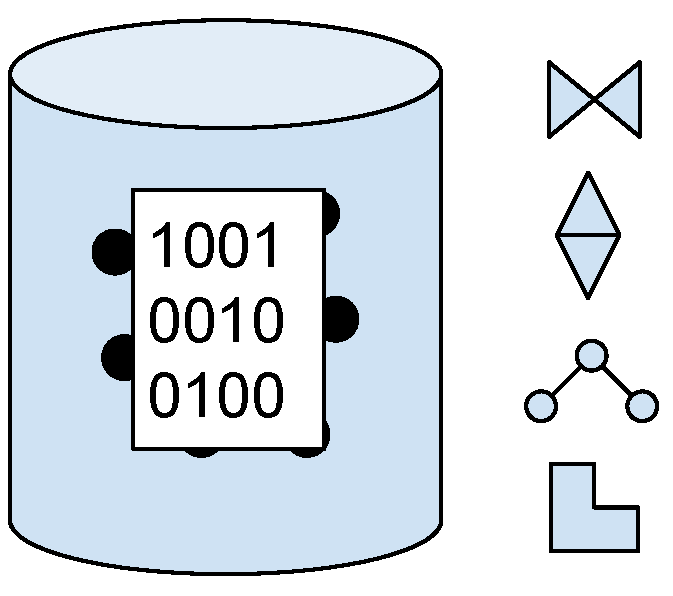
\includegraphics[scale=0.4]{figs/cvl-code-to-data-exploit.pdf}
%	\end{figure}       
%	\end{center}                     
%}


%\frame[t]
%{
%  \frametitle{The problem in a nutshell}
%  \begin{itemize}[<+->]
%  \item User assigns a \emph{weight} to records using an SQL expression
%  \item User-defined \emph{spatial constraints} that apply are listed with parameters
%  \item \emph{Minimize} combined weight of non-visible records
%  \vspace{1em}
%  \end{itemize}
%  	\begin{columns}[t]
%		\begin{column}[l]{5cm}
%  		\includegraphics<1,2>[scale=0.385]{figs/cvl-weight.pdf}
%		\end{column}
%		\begin{column}[r]{4cm}
%		\includegraphics<2>[scale=0.25]{figs/cvl-rules-rules.pdf}
%		\end{column} 
%  	\end{columns}
%}




%\frame{
%	\frametitle{Expressing constraints in our programming language}
%	\begin{itemize}[<+->]
%	\item How to express constraints in the high-level language?
%	\end{itemize}
%	\begin{center}
%	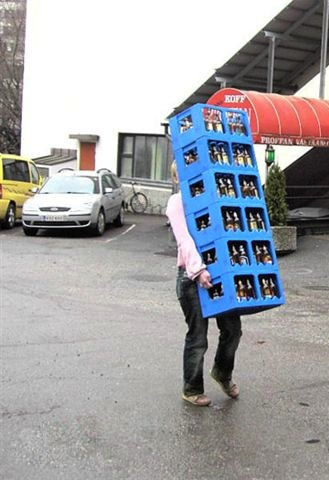
\includegraphics[scale=0.3]{figs/divisionoflabour2.jpg}
%	\end{center}
%}


%\frame{
%	\frametitle{Conflict sets}
%	\begin{itemize}[<+->]
%	\item Group violating records by  ``conflict set''
%	\item Conflict set is subset of records that can not all be visible on same zoom level
%	\item Some of these records must be filtered out
%	\item Which ones is decided by an algorithm
%	\end{itemize}
%	\begin{center}
%	\begin{figure}
%    		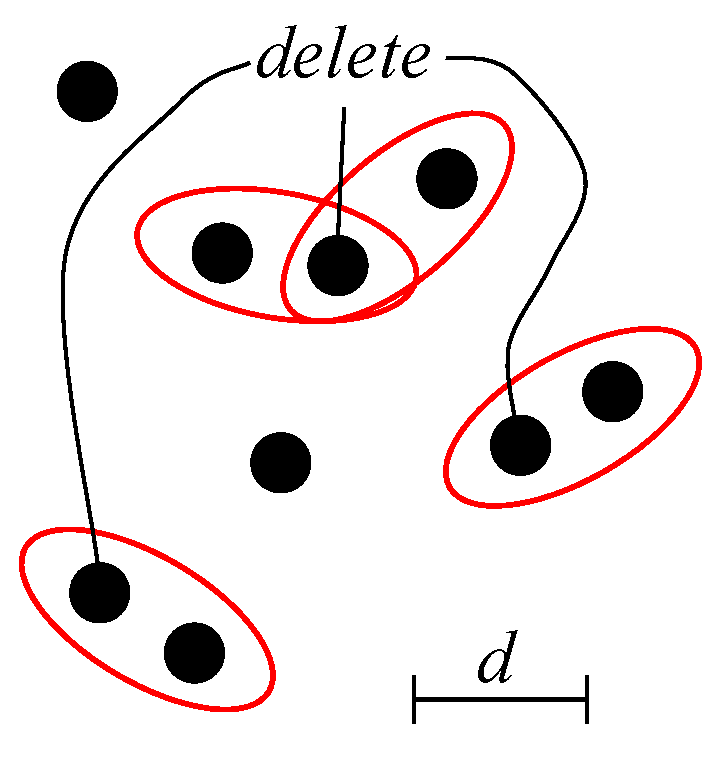
\includegraphics[scale=0.3]{figs/cvl-proximity-conflicts-2.pdf}
%	\end{figure}       
%	\end{center}
%}

\begin{frame}[fragile]
\frametitle{High-level language: \texttt{CREATE CONSTRAINT} statement}
\begin{lstlisting}[escapechar=@]
CREATE CONSTRAINT Proximity @\pause@

AS NOT EXISTS ( -- @reuse SQL to finds conflicts@ @\pause@
  SELECT  
    l.id || r.id AS conflictID, 
    Unnest(array[l.id, r.id]) AS recordID @\pause@
  FROM
    {level_view} l JOIN {level_view} r @\pause@
  ON
    l.id < r.id @\pause@
  AND
    l.geom && ST_Expand(r.geom, 
      CVL_Resolution({z}, 256) * {parameter_1}) @\pause@
  AND
    ST_Distance(l.geom, r.geom) < 
      CVL_Resolution({z}, 256) * {parameter_1} 
) @\pause@
RESOLVE IF DELETE (1)
\end{lstlisting}
\end{frame}


\frame[t]
{
	\frametitle{Crash course on bi-partite graphs}
	\begin{itemize}[<+->]
	\item Graph = $nodes$ and $edges$
	\item ``Bi-partite'' graph is a \emph{restricted} graph
	\item nodes on $left$ and nodes on $right$ (e.g. organizing a dance)
	\end{itemize}
	\vspace{1em}
	\begin{center}
  		\includegraphics<1>[scale=1]{figs/cvl-general-graph.pdf}
		\includegraphics<3>[scale=1]{figs/cvl-bipartite-graph-0.pdf}
  	\end{center}
}


\frame[t]
{
	\frametitle{Constraints and bi-partite graphs}
	\begin{itemize}[<+->]
	\item A record can be in several conflicts
	\item A conflict involves several records
	\item Corresponds to ``bi-partite graph'':
	\end{itemize}
	\vspace{1em}
	\begin{center}
	\begin{figure}
		\includegraphics<1,2>[scale=0.30]{figs/cvl-proximity-conflicts-1.pdf}
  		\includegraphics<3>[scale=0.8]{figs/cvl-bipartite-graph.pdf}
	%\caption{Bi-partite graph for proximity constraint}
	\end{figure}
  	\end{center}
}

\frame[t]
{
	\frametitle{Compute solution using bi-partite graphs}
	\begin{itemize}[<+->]
	\item Records have weights (e.g. restaurant star-rating)
	\item Conflicts are resolved by ``deleting'' records ($1$ for proximity constraint)
	\item \textbf{Problem}: Pick minimum weight set of records on left \\that resolves all conflicts on right
	\item Optimal solution has cost $6$
	\end{itemize}
	\vspace{1em}
	\begin{center}
	\begin{figure}
  		\includegraphics<1>[scale=0.8]{figs/cvl-bipartite-graph-weighted.pdf}
		\includegraphics<2,3>[scale=0.8]{figs/cvl-bipartite-graph-weighted-b.pdf}
		\includegraphics<4>[scale=0.8]{figs/cvl-bipartite-graph-weighted-2.pdf}
	\caption{Bi-partite graph for proximity constraint}
	\end{figure}
  	\end{center}
}

\frame{
	\frametitle{Recycle technology: algorithms}
	\begin{center}
	
\includegraphics[scale=0.88]{figs/wall-e.jpg}
	\end{center}
}

\frame[t]
{
	\frametitle{Set multicover problem}
	\begin{itemize}[<+->]
	\item This problem is known as \emph{set multicover problem} (SMCP)
	\item Several good algorithms exist for this problem
	\item We implemented a few of them inside the database
	\item \emph{Drawback}: SMCP is $\mathcal{NP}$-hard
	\item \emph{Maybe OK}: generalization problem may also be $\mathcal{NP}$-hard
	\end{itemize}
	\vspace{1em}
	\begin{center}
  		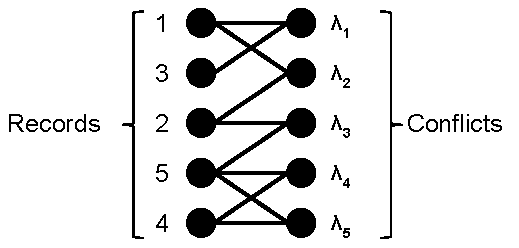
\includegraphics[scale=0.8]{figs/cvl-set-multicover-graph.pdf}
  	\end{center}
}

\frame[t]
{
	\frametitle{General algorithm}
	\begin{itemize}[<+->]
	\item Solve the generalization problem using ``ladder'' approach
	\item On each zoom level solve an instance of SMCP
	\item Solution to SMCP are the records that are filtered out
	\item Remaining records are ``copied'' to next lower zoom-level
	\vspace{1em}
	\end{itemize}
	\begin{center}
  		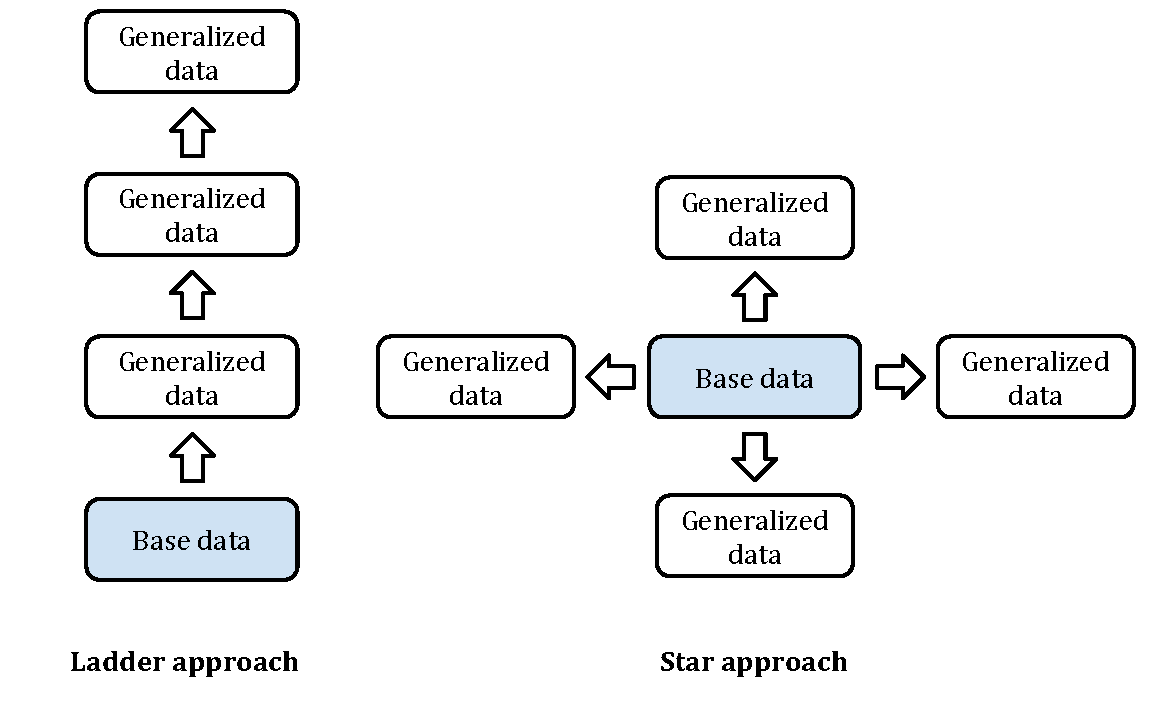
\includegraphics[scale=0.4]{figs/cvl-star-and-ladder.pdf}
  	\end{center}
}

\frame
{
	\frametitle{Experiments}
	\begin{itemize}[<+->]
	\item We conducted experiments on Amazon EC2
	\item PostgreSQL 9.2.4 with PostGIS 2.0, GDAL 1.9.2, Python 2.6.8
	\item Data: Openflights, OpenStreetMap and Danish Geodata Agency
	\item Tested with both point, line and polygon datasets
	\item POI (500K points), Rivers (2M points), Zones (9M points)
	\end{itemize}
}

\frame
{
	\frametitle{Performance breakdown}


\begin{figure}[tb]
  \begin{minipage}{0.45\linewidth}
    \centerline{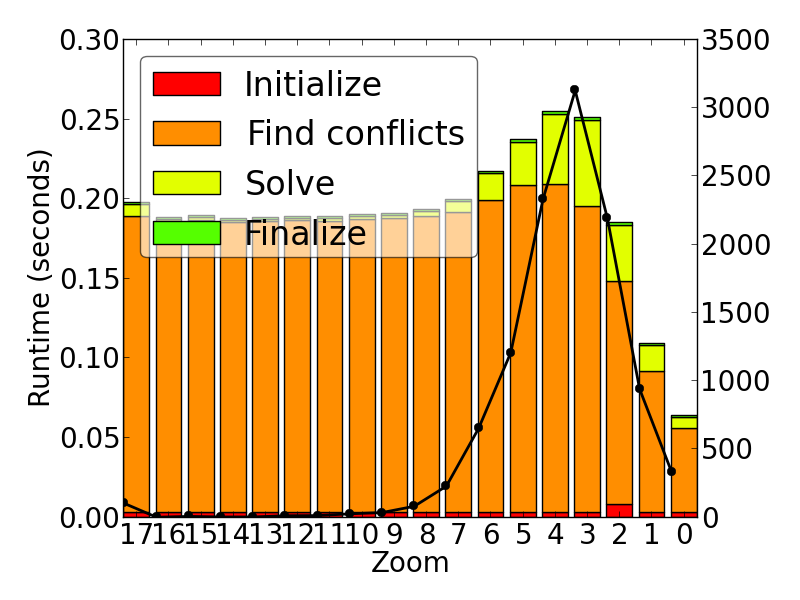
\includegraphics[width=1\linewidth]{./figs/prelim_pnt_7k_airports_heuristic_B.png}}
    \centerline{(a) SGA + Proximity}
  \end{minipage} \hfill
  \begin{minipage}{0.45\linewidth}
    \centerline{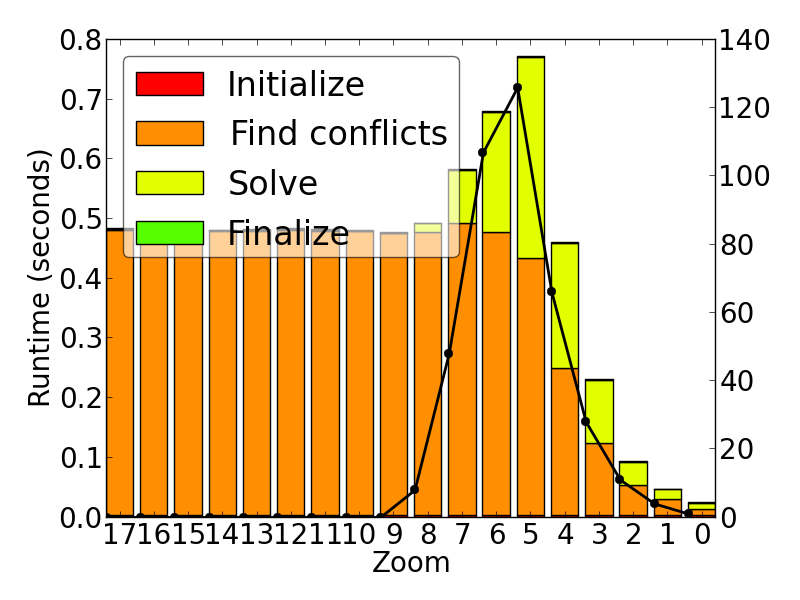
\includegraphics[width=1\linewidth]{./figs/prelim_pnt_7k_airports_lp_A.png}}
    \centerline{(b) LPGA + Visibility}
  \end{minipage}
  %\vspace{-1ex}
  \caption{Performance breakdown by zoom level (7K airports). Black line is number of conflicts}
  \label{fig:performance:breakdown}
  \vspace{-2ex}
\end{figure}

	
	
}

\frame
{
	\frametitle{Results for point and polygon data}
\begin{table}[htdp]
\vspace{-2ex}
\begin{center}
\begin{tabular}{|c|c|c|r|r|}
\hline
\textbf{Dataset} & \textbf{Constraint} & \textbf{Solver} & \textbf{Time} & \textbf{Qual.}\\ 
\hline
Points (7K)  & Visibility & SGA & 7s & 1.0 \\
Points (500K) & Visibility & SGA & 6m 9s & 1.0 \\
Points (7K)  & Proximity  & SGA & 3s & 1.18 \\
Points (500K) & Proximity & SGA & 7m 17s & 1.21 \\
\hline
Lines (2M) & Visibility & SGA & 1h 32m & 1.36 \\
Polygons (9M) & Visibility & SGA & 13m 38s & 1.20 \\
Lines (2M)  & Proximity  & SGA& 1h 11m s & 1.46 \\
Polygon (9M) & Proximity & SGA & 4h 28m & 1.72 \\
\hline
\end{tabular}
\end{center}
\caption{Decent quality + running time in seconds, minutes or hours}
\label{tab:complex:overview}
\vspace{-6ex}
\end{table}%


}

%\frame[t]
%{
%  \frametitle{Computing solutions}
%	\begin{itemize}[<+->]
%	\item Use SQL from first part of constraint definition to find sets of violating records
%	\item Use SQL from second part of constraint definition to find out how many records should be filtered out
%	\item Use an algorithm to select the records
%	\end{itemize}
%	
%	\begin{center}
%	\begin{figure}
%  		\fbox{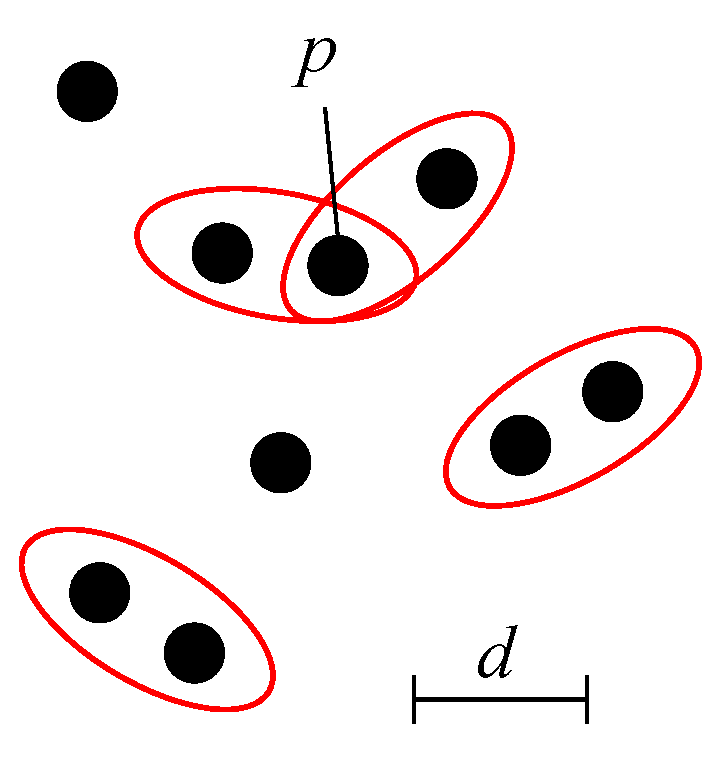
\includegraphics[scale=0.25]{figs/cvl-proximity-conflicts.pdf}}
%	\caption{Four conflict sets generated by a proximity constraint}
%	\end{figure}
%  	\end{center}
%}
%
%\frame[t]
%{
%  \frametitle{Computing solutions}
%	\begin{itemize}[<+->]
%	\item Combination of record weights and spatial constraints (proximity, density) present a natural optimization problem
%	\item Mapping to set multicover problem (SMP)
%	\item Reuse existing algorithms for SMP (database implementations)
%	\end{itemize}
%	\begin{center}
%  		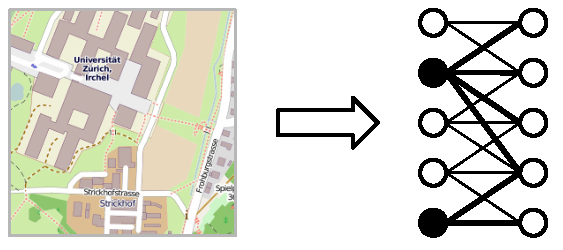
\includegraphics[scale=0.70]{figs/cvl-spatial-to-nonspatial.pdf}
%  	\end{center}
%}

\frame[t]
{
  \frametitle{Summary}
	\begin{itemize}
	\item Designed a high-level language for generalization called CVL
	\item Compiled to low-level database program and moved code-to-data
	\item Exploited correspondence to well-known optimization problem
	\end{itemize}
}

\frame[t]
{
  \frametitle{Future work}
  	\begin{center}
  	\fbox{We need your help :-)}
	\end{center}
	\begin{itemize}
	\item Implement aggregation as generalization operator
	\item Validate method in user tests
	\item More ``pure'' SQL implemention
	\item Improve running time, move towards real-time
	\end{itemize}
	\begin{center}
	\begin{figure}
  		\fbox{Thank you!}
	\end{figure}
	\end{center}
	\begin{center}
	  	Work will appear at ICDE '14 in Chicago, IL
	\end{center}	
}


\end{document}